\begin{figure}[htbp]
\centering
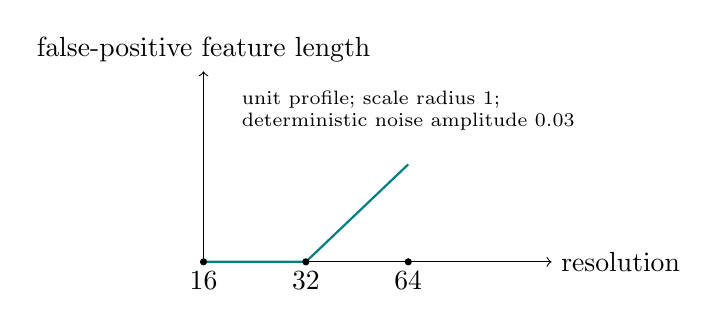
\begin{tikzpicture}[x=1.3cm,y=1.1cm]
\draw[->] (0,0) -- (3.4,0) node[right]{resolution};
\draw[->] (0,0) -- (0,2.2) node[above]{false-positive feature length};
\draw[teal,thick] (0,0.000) -- (1,0.000) -- (2,1.125);
\foreach \x/\n in {0/16,1/32,2/64} {\fill (\x,0) circle (1.3pt); \node[below] at (\x,0) {\n};}
\node[align=left,font=\scriptsize] at (2.0,1.75) {unit profile; scale radius $1$;\\deterministic noise amplitude $0.03$};
\end{tikzpicture}
\caption{Generated scale-stability summary for the deterministic unit-profile ridge/valley proxy. The vertical quantity is a one-dimensional support-length proxy, not a surface ridge arc length.}
\label{fig:vii42-c16-scale-stability}
\end{figure}
